\documentclass[10pt, aspectratio=169]{beamer}
\usepackage[russian]{babel}
\usepackage{pgfpages}
\usepackage{graphicx}
\usepackage{tabularx}
\usepackage[T1]{fontenc}
\usepackage{tgbonum}

\setbeameroption{hide notes}
\setbeamertemplate{footline}{
    \leavevmode
    \begin{beamercolorbox}[ht=2.5ex,dp=1.125ex,leftskip=1em,rightskip=.3em]{author in head/foot}
        \usebeamerfont{author in head/footer}Алтунина Екатерина Юрьевна
        \hfill
        \usebeamerfont{page number in head/foot}\insertframenumber\,/\,\inserttotalframenumber\hspace{1em}
    \end{beamercolorbox}
    \vspace{0.2em}
}
% TITLE PAGE
\title[Short title]{Визуализация теней в реальном времени }
\date[02.02.2026]{Апрель, 2026}
\author[author]{Алтунина Екатерина Юрьевна}
\institute{Руководитель: Романов Алексей Алексеевич\and ИПКН ИТМО, программа «Разработка программного обеспечения»\and(Санкт-Петербург)}


% \setbeamerfont{normal text}{family=\sffamily}
% \setbeamerfont{structure}{family=\sffamily}

\begin{document}
%_____________________________________________________
% Title page
\frame[plain]{
\titlepage
}
%_____________________________________________________
% ToC
% \frame{{Содержание}
% \tableofcontents
% }
%_____________________________________________________
% 
\section{Section 1}
\subsection{Subsection 1.1}
\frame{{Введение в предметную область} 

\begin{columns}
    \column{0.65\textwidth}
    Тени - ключевой элемент любой системы визуализации: 
    они определяют расстояния между объектами, особенно в картографии.

    В условиях веб-браузера приходится находить разумный 
    компромисс между реалистичностью теней и скоростью работы сцены.
    \column{0.3\textwidth}
    
\includegraphics[width=\textwidth]{figures/no shadows.PNG}
    
\includegraphics[width=\textwidth]{figures/shadows.PNG}
\end{columns}
}

\subsection{Subsection 1.2}
\frame{{Существующие решения} 

\begin{table}[h]
\centering
\footnotesize
\begin{tabular}{|l|c|c|c|c|c|c|}
\hline
\textbf{Метод} & \textbf{Скорость} & \textbf{Память} & \textbf{Область}  & \textbf{Дин. объекты} & \textbf{Вывод} \\
\hline
Планарные тени    & + & + & - & - & + & Малая обл. применения \\
\hline
Теневой объем     & {\tiny$\pm$} & {\tiny$\pm$} & + & + & - & Зависит от покрытых пикселей \\
\hline
Трассировка лучей & - & - & + & + & - & Высокая сложность \\
\hline
Карты теней       & + & {\tiny$\pm$} & + & {\tiny$\pm$} & {\tiny$\pm$} & \textbf{Используем для статич. объектов} \\
\hline
Аналитические тени       & + & + & + & + & + & \textbf{Используем для дин. объектов} \\
\hline
\end{tabular}
\caption{Сравнение методов рендеринга теней}
\end{table}

}

\subsection{Subsection 1.3}
\frame{{Карты теней}

\begin{columns}
\column{0.5\textwidth}
    \centering
    Решение, основанное на построении карты глубины со стороны источника света
    \vspace{0.5em}
    \begin{itemize} 
        \item (+) Для различных источников света
        \item (+) Предсказуемы в плане оценки стоимости построения карты теней
        \item (+) Карту теней можно переиспользовать
        \item (--) Наличие артефактов
        \item (--) Иногда надо много карт теней
        \item (--) Невозможность построить тень для объекта, отбрасывающего тень в затененной области
        \item (--) Базово не поддерживают мягкие тени
    \end{itemize}
\column{0.5\textwidth}
    \centering
    
\includegraphics[width=0.6\textwidth]{figures/shadowmaps-shadows.png}
\end{columns}

}

\subsection{Subsection 1.7}
\frame{{Аналитические тени}

\begin{columns}
\column{0.5\textwidth}
    \centering
    Решение, основанное на аппроксимации модели более простыми фигурами
    \vspace{0.5em}
    \begin{itemize} 
        \item (+) Быстрое решение
        \item (+) Мягкие тени
        \item (+) Мало памяти
        \item (--) Нужно аппроксимировать модель
        \item (--) Время работы зависит от количества примитивов
        \item (--) Возможность затенить области, уже подверженные влиянию теней.
    \end{itemize}
\column{0.5\textwidth}
    \centering
    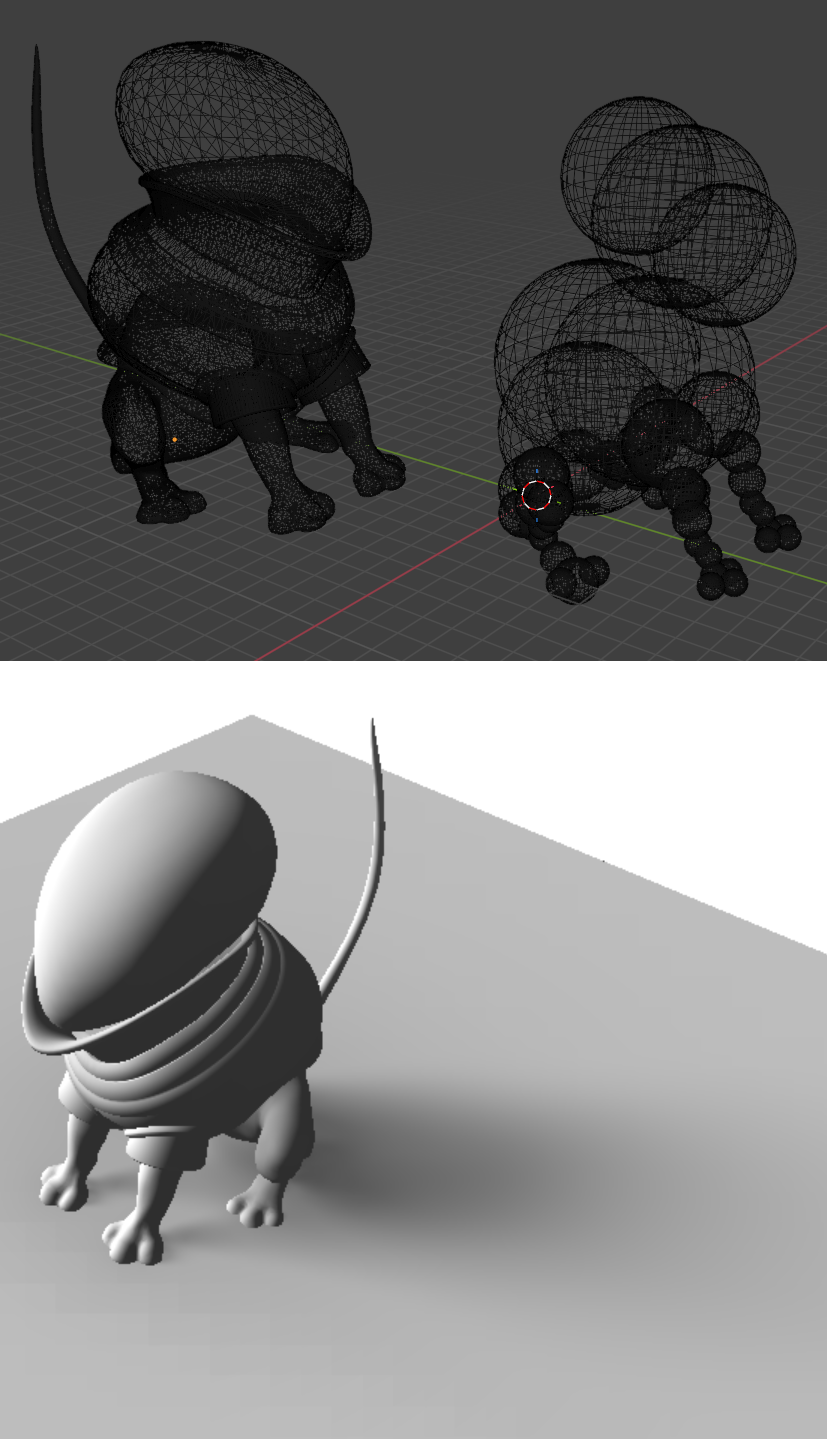
\includegraphics[width=0.6\textwidth]{figures/analytic-shadows.PNG}
\end{columns}

}

%_____________________________________________________
%
\section{Section 2}
\subsection{Subsection 2.1}
\frame{{Цель и задачи} 
{} 

\textbf{Цель работы:} оценить применимость и производительность метода аналитических теней для отрисовки динамических объектов в браузере.
\vspace{1em}

\textbf{Задачи:}
\begin{enumerate}
    \item Создать Web-песочницу с использованием WebGPU, реализовать классический подход к визуализации теней - карту теней.
    \item Реализовать метод аналитических теней для динамических объектов на произвольных геометрических формах и предусмотреть возможность изменения параметров, влияющих на отрисовку теней.
    \item Провести анализ производительности и визуально оценить качество предложенного решения. 
\end{enumerate}
}

\section{Section 3}
\subsection{Subsection 3.1}
\frame{{Реализация карты теней} 

\hspace{1cm}% Adjust the length as needed
\begin{columns}
\column{0.5\textwidth}
    На первом этапе разработки:
    \vspace{0.5em}
    \begin{itemize} 
        \item Реализована навигация по сцене с двумя видами камер (для работы с камерой и навигацией - Three.js)
        \item Реализован метод каскадных теней (до 8 каскадов)
        \item Динамический расчет границ отсечения каскадов в зависимости от положения камеры
    \end{itemize}
\column{0.5\textwidth}
    \hfill
    \left.
    
\includegraphics[width=1.0\textwidth]{figures/casc.png}
    \right\

\end{columns}

}

\section{Section 3}
\subsection{Subsection 3.3}
\frame{{Борьба с артефактами} 
{}

\vspace{0.5em}
\begin{table}[h]
    \centering
    \begin{tabular}{ccc}
        \textbf{Алиасинг} & \textbf{Самозатенение} & \textbf{Большое смещение} \\
        \parbox{0.3\textwidth}{\centering Cтупенчатости границы тени, дрожание линии теней} &
        \parbox{0.3\textwidth}{\centering Фрагмент ошибочно затеняет сам себя} &
        \parbox{0.3\textwidth}{\centering Тень «отрывается» от объекта} \\
        
\includegraphics[width=0.3\textwidth]{figures/pcf.png} & 
        
\includegraphics[width=0.3\textwidth]{figures/zfighting.png} & 
        
\includegraphics[width=0.3\textwidth]{figures/peterpanning.png} \\
        \parbox{0.3\textwidth}{\centering \textbf{Метод борьбы:} PCF (Percentage Closer Filtering) --- Сглаживание краёв} & 
        \parbox{0.3\textwidth}{\centering \textbf{Метод борьбы:} Смещение (depth bias)} & 
        \parbox{0.3\textwidth}{\centering \textbf{Метод борьбы:} Отсечение лицевых полигонов} \\
    \end{tabular}
\end{table}




}

\section{Section 3}
\subsection{Subsection 3.5}
\frame{{Аналитические тени} 
{}

}

\subsection{Subsection 3.6}
\frame{{Тайлинг при использовании аналититческих теней} 
{}


}

\subsection{Subsection 3.7}
\frame{{Получение на этапе рендеринга} 
{}

}

\subsection{Subsection 3.8}
\frame{{Комбинация методов} 
{}

Пайплайн построения теней для сцены с динамическими объектами при использовании карт теней устроен так:
\begin{itemize} 
    \item При изменении положения камеры идет перестройка карты теней для статических объектов
    \item При изменен
\end{itemize}

}

\subsection{Subsection 3.8}
\frame{{Валидация} 
{}


}

\section{Section 4}
\subsection{Subsection 4.1}
\frame{{Вывод} 
{}

На данный момент:

\begin{itemize}  
\item Есть работающая песочница. Реализован классический метод каскадных теней.
\item Разработана система для разделения статических и динамических объектов.
\item Начата работа по имплементации аналитических теней.
\end{itemize}

}

\subsection*{Section 5}
\frame{{Карты теней} 

Алгоритм:
\begin{itemize} 
\item Сначала происходит построение сцены в Z-буфер с точки зрения источника света, 
чтобы установить видимые из этой точки пикселы и расстояния до них. 
\item После этого сцена перестраивается уже с точки зрения наблюдателя. 
\item Если пиксель невидим с точки зрения источника света, он закрашивается тёмным цветом.
\end{itemize}
\begin{columns}
    \column{0.3\textwidth}
    
\includegraphics[width=\textwidth]{depthmap.PNG}
    \column{0.3\textwidth}
    
\includegraphics[width=\textwidth]{shadows.PNG}
\end{columns}
}

\subsection*{Section 6}
\frame{{Аналитические тени}

\vspace{0.5em}
\begin{columns}
    \column{0.3\textwidth}
    Алиасинг
    
\includegraphics[width=\textwidth]{aliasing-no-pcf.jpg}
    \column{0.3\textwidth}
    <<Теневые прыщи>>
    
\includegraphics[width=\textwidth]{shadow-acne.jpg}
    \column{0.3\textwidth}
    Обрезание теней
    
\includegraphics[width=\textwidth]{cutoutshadows.jpg}
\end{columns}
}

\end{document}